\documentclass[a4paper,14pt]{extarticle}

\usepackage[utf8x]{inputenc}
\usepackage[T1,T2A]{fontenc}
\usepackage[russian]{babel}
\usepackage{hyperref}
\usepackage{indentfirst}
\usepackage{here}
\usepackage{array}
\usepackage{graphicx}
\usepackage{caption}
\usepackage{subcaption}
\usepackage{chngcntr}
\usepackage{amsmath}
\usepackage{amssymb}
\usepackage{pgfplots}
\usepackage{pgfplotstable}
\usepackage[left=2cm,right=2cm,top=2cm,bottom=2cm,bindingoffset=0cm]{geometry}
\usepackage{multicol}

\renewcommand{\le}{\ensuremath{\leqslant}}
\renewcommand{\leq}{\ensuremath{\leqslant}}
\renewcommand{\ge}{\ensuremath{\geqslant}}
\renewcommand{\geq}{\ensuremath{\geqslant}}
\renewcommand{\epsilon}{\ensuremath{\varepsilon}}
\renewcommand{\phi}{\ensuremath{\varphi}}

\counterwithin{figure}{section}
\counterwithin{equation}{section}
\counterwithin{table}{section}
\newcommand{\sign}[1][5cm]{\makebox[#1]{\hrulefill}} % Поля подписи и даты
\graphicspath{{pics/}} % Путь до папки с картинками
\captionsetup{justification=centering,margin=1cm}
\def\arraystretch{1.3}

\begin{document}	% начало документа

\begin{titlepage}
\begin{center}
	\textbf{Санкт-Петербургский Политехнический Университет \\Петра Великого}\\[0.3cm]
	\small Институт компьютерных наук и технологий \\[0.3cm]
	\small Кафедра компьютерных систем и программных технологий\\[4cm]
	
	\textbf{ОТЧЕТ}\\ \textbf{о лабораторной работе}\\[0.5cm]
	\textbf{<<Исследование частотных характеристик пассивных RC-цепей>>}\\[0.1cm]
	\textbf{Электротехника и Электроника}\\[10.5cm]
\end{center}

\begin{flushright}
	\begin{minipage}{0.60\textwidth}
		\begin{flushleft}
			\small \textbf{Работу выполнили студенты}\\[3mm]
			\small группа 23501/4 \hspace*{17mm} Дьячков В.В.\\[3mm]
			\small группа 23501/4 \hspace*{17mm} Ламтев А.Ю.\\[5mm]
			
			\small \textbf{Преподаватель}\\[5mm]
		 	\small \sign[3.5cm] \hspace*{8mm} к.т.н., доц. Кочетков Ю.Д.\\[0.5cm]
		\end{flushleft}
	\end{minipage}
\end{flushright}

\vfill

\begin{center}
	\small Санкт-Петербург\\
	\small \the\year
\end{center}
\end{titlepage}


\section{Цель работы}
Исследовать процессы, происхожящие в дифференцирующей и интегрирующей RC-цепях при подаче на вход однополярного прямоугольного импульса.

\section{Чертеж схемы исследуемого устройства}
\begin{figure}[h]
\centering
\begin{subfigure}[b]{0.35\textwidth}
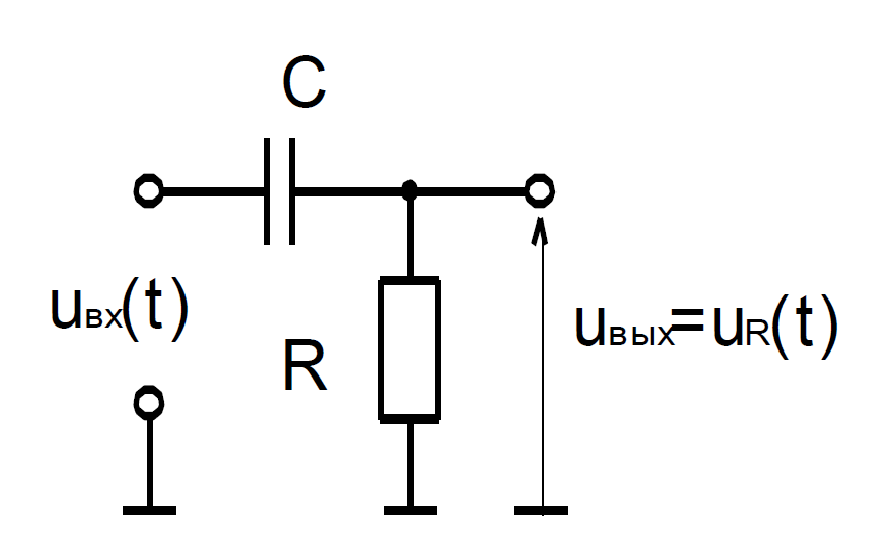
\includegraphics[scale=0.27]{diff.png}
\caption{Дифференцирующая\\ цепь}\label{figure:2.1:a}
\end{subfigure}
\begin{subfigure}[b]{0.35\textwidth}
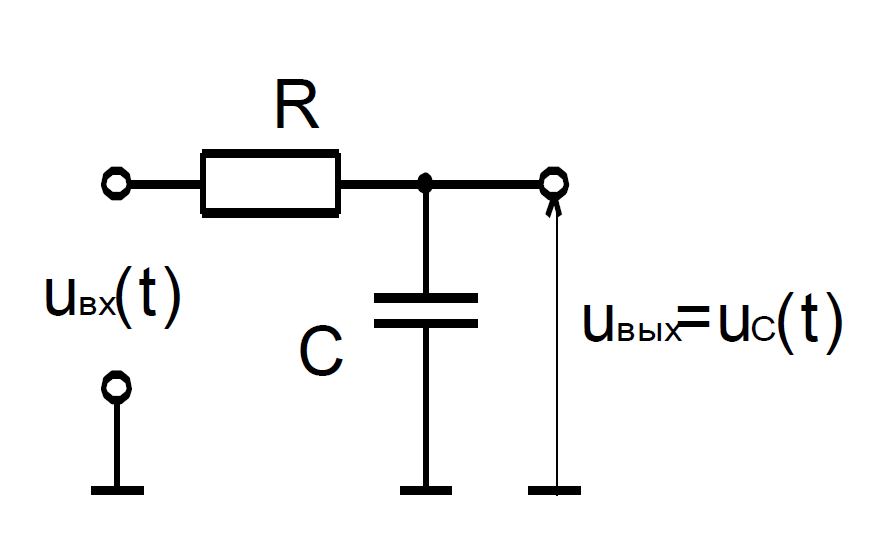
\includegraphics[scale=0.27]{int.png}
\caption{Интегрирующая\\ цепь}\label{figure:2.1:b}
\end{subfigure}
\end{figure}

На рисунке \ref{figure:2.1:a} изображена дифференцирующая RC-цепь, на \ref{figure:2.1:b} - интегрирующая RC-цепь.


\section{Исходные данные}

Исходные значения были выбраны как в таблице \ref{tab:3:1}:

\begin{table}[H]
	\begin{center}
	\caption{Исходные данные}
	\def\arraystretch{1.5}
		\begin{tabular}{|c|c|c|c|c|c|c|}
			\hline 
			№ & Тип цепи & $U_\text{имп}$, B & R, кОм & С, нФ & $t_\text{имп}$, $\mu c$ & Q\\ 
			\hline 
			1 & Дифф & 10 & 10 & 0.1 & 10 & 10\\ 
			\hline 
			2 & Дифф & 10 & 10 & 1 & 10 & 10\\ 
			\hline 
			3 & Дифф & 10 & 10 & 10 & 10 & 10\\ 
			\hline 
			4 & Инт & 10 & 10 & 0.1 & 10 & 10\\ 
			\hline 
			5 & Инт & 10 & 10 & 1 & 10 & 10\\ 
			\hline 
			6 & Инт & 10 & 10 & 10 & 10 & 10\\
			\hline 
			7 & Инт & 10 & 10 & 10 & 10 & 5\\ 
			\hline 
			8 & Инт & 10 & 10 & 10 & 10 & 3\\ 
			\hline
		\end{tabular}
		\label{tab:3:1}
	\end{center}
\end{table}

\section{Теоретические зависимости}

Рассчитаем теоретические занчения $U_R(t)$ и $U_C(T)$ для дифференцирующей и интегрирующей RC-цепей.

\subsection{Расчетные формулы}

\begin{itemize}

\item Входное напряжение:
\begin{equation}
U_\text{вх} = \{(0 \text{ при } t < 0); (U_\text{имп} \text{ при } 0 \leq t \leq t_\text{имп}); (0 \text{ при } t \geq t_\text{имп})\}
\end{equation}

\item Выходное напряжение:

\begin{enumerate}
\item Для дифференцирующей цепи
\begin{equation}
U_R(t) = [U_C(\infty) - U_C(0)] \cdot e^{-\frac{t}{\tau}}
\end{equation}

\item Для интегрирующей цепи
\begin{equation}
U_C(t) = [U_C(0) - U_C(\infty)] \cdot e^{-\frac{t}{\tau}} + U_C(\infty)
\end{equation}

\end{enumerate}
\end{itemize}

\subsection{Расчеты для дифференцирующей RC-цепи}

\subsubsection{C = 0.1 нФ}

		$\tau = R \cdot C = 10 \cdot 10^3 \cdot 0.1 \cdot 10^{-9} = 10^{-6}$ (c)
		
		$t_\text{имп} = 10^{-5}$ (c)
		
\begin{itemize}
\item[] а) этап заряда конденсатора

		$U_C(0)	= 0,\ \ U_C(\infty) = U_\text{имп}$\\
		$U_R(t) = [U_\text{имп} - 0] \cdot e^{-\frac{t}{\tau}} = [10 - 0] \cdot e^{-\frac{t}{10^{-6}}} = 10 \cdot e^{-\frac{t}{10^{-6}}}$\\
		$U_R(0) = 10 \cdot e^{-\frac{0}{10^{-6}}} = 10 \cdot e^0 = 10$ (В)\\
		$U_R(t_\text{имп}) = 10 \cdot e^{-\frac{10^{-5}}{10^{-6}}} = 10 \cdot e^{-10} = 0$ (В)\\

\item[] б) этап разряда конденсатора
		
		$U_C(0)	= U_\text{имп},\ \ U_C(\infty) = 0$\\		
		$U_R(t) = [0 - U_\text{имп}] \cdot e^{-\frac{t}{\tau}} = [0 - 10] \cdot e^{-\frac{t}{10^{-6}}} = -10 \cdot e^{-\frac{t}{10^{-6}}}$\\
		$U_R(0) = -10 \cdot e^{-\frac{0}{10^{-6}}} = -10 \cdot e^0 = -10$\\
		Выберем такое $t$, что $t \gg \tau$, например, $t = 10 \cdot \tau$ \\
		$U_R(10 \cdot \tau) = -10 \cdot e^{-\frac{10^{-5}}{10^{-6}}} = -10 \cdot e^{-10} = 0$ (В)\\
		
\end{itemize}

\subsubsection{C = 1 нФ}

		$\tau = R \cdot C = 10 \cdot 10^3 \cdot 10^{-9} = 10^{-5}$ (c)
		
		$t_\text{имп} = 10^{-5}$ (c)

\begin{itemize}
\item[] а) этап заряда конденсатора

		$U_C(0)	= 0,\ \ U_C(\infty) = U_\text{имп}$\\
		$U_R(t) = [U_\text{имп} - 0] \cdot e^{-\frac{t}{\tau}} = [10 - 0] \cdot e^{-\frac{t}{10^{-5}}} = 10 \cdot e^{-\frac{t}{10^{-5}}}$\\
		$U_R(0) = 10 \cdot e^{-\frac{0}{10^{-5}}} = 10 \cdot e^0 = 10$ (В)\\
		$U_R(t_\text{имп}) = 10 \cdot e^{-\frac{10^{-5}}{10^{-5}}} = 10 \cdot e^{-1} = 3.679$ (В)\\

\item[] б) этап разряда конденсатора

		$U_C(0)	= U_\text{имп} - U_R(t),\ \ U_C(\infty) = 0$\\
		$U_R(t) = [0 - (U_\text{имп} - U_R(t))] \cdot e^{-\frac{t}{\tau}} = [0 - (10 - 3.679)] \cdot e^{-\frac{t}{10^{-5}}} = -6.32 \cdot e^{-\frac{t}{10^{-5}}}$\\
		$U_R(0) = -6.321 \cdot e^{-\frac{0}{10^{-5}}} = -6.321 \cdot e^0 = -6.321$ (В)\\
		Выберем такое $t$, что $t \gg \tau$, например, $t = 10 \cdot \tau$ \\
		$U_R(10 \cdot \tau)	= -6.321 \cdot e^{-\frac{10^{-4}}{10^{-5}}} = -6.321 \cdot e^{-10} = 0$ (В)\\
		
\end{itemize}

\subsubsection{C = 10 нФ}

		$\tau = R \cdot C = 10 \cdot 10^3 \cdot 10 \cdot 10^{-9} = 10^{-4}$ (c)
		
		$t_\text{имп} = 10^{-5}$ (c)

\begin{itemize}
\item[] а) этап заряда конденсатора

		$U_C(0)	= U_\text{имп},\ \ U_C(\infty) = 0$\\		
		$U_R(t) = [0 - U_\text{имп}] \cdot e^{-\frac{t}{\tau}} = [10 - 0] \cdot e^{-\frac{t}{10^{-4}}} = 10 \cdot e^{-\frac{t}{10^{-4}}}$\\
		$U_R(0) = 10 \cdot e^{-\frac{0}{10^{-4}}} = 10 \cdot e^0 = 10$ (В)\\
		$U_R(t_\text{имп}) = 10 \cdot e^{-\frac{10^{-5}}{10^{-4}}} = 10 \cdot e^{-0.1} = 9.048$ (В)\\

\item[] б) этап разряда конденсатора
		
		$U_C(0)	= U_\text{имп} - U_R(t),\ \ U_C(\infty) = 0$\\
		$U_R(t) = [0 - (U_\text{имп} - U_R(t))] \cdot e^{-\frac{t}{\tau}} = [0 - (10 - 9.048)] \cdot e^{-\frac{t}{10^{-4}}} = -0.952 \cdot e^{-\frac{t}{10^{-4}}}$\\
		$U_R(t) = -0.952 \cdot e^{-\frac{0}{10^{-4}}} = -0.952 \cdot e^0 = -0.952$ (В)\\
		Выберем такое $t$, что $t \gg \tau$, например, $t = 10 \cdot \tau$ \\
		$U_R(t) = -0.952 \cdot e^{-\frac{10^{-3}}{10^{-4}}} = -0.952 \cdot e^{-10} = 0$ (В)\\
		
\end{itemize}

\subsection{TODO Расчеты для интегрирующей RC-цепи}

\subsubsection{C = 0.1 нФ, Q = 10}

		$\tau = R \cdot C = 10 \cdot 10^3 \cdot 0.1 \cdot 10^{-9} = 10^{-6}$ (c)
		
		$t_\text{имп} = 10^{-5}$ (c)
		
		$Q = 10$		
		
		$t_\text{п} = Q \cdot t_\text{имп} = 10 \cdot 10^{-5} = 10^{-4}$ (c)
\begin{itemize}
\item[] а) этап заряда конденсатора

		$U_C(0) = 0,\ \ U_C(\infty) = U_\text{имп}$\\
		$U_C(t) = [0 - U_\text{имп}] \cdot e^{-\frac{t}{\tau}} + U_\text{имп} = -10 \cdot e^{-\frac{t}{10^{-6}}} + 10$\\
		$U_C(0) = -10 \cdot e^{-\frac{0}{10^{-6}}} + 10 = -10 \cdot e^0 + 10 = 0$ (В)\\
		$U_C(t_\text{имп}) = -10 \cdot e^{-\frac{10^{-5}}{10^{-6}}} + 10 = -10 \cdot e^{-10} + 10 = 10$ (В)\\

\item[] б) этап разряда конденсатора
		
		$\frac{\tau}{t_\text{имп}} = \frac{10^{-6}}{10^{-5}} = 0.1 < 0.33 \Rightarrow U_C(0) = U_\text{имп},\ \ U_C(\infty) = 0$\\
		$U_C(t) = [U_\text{имп} - 0] \cdot e^{-\frac{t}{\tau}} + 0 = 10 \cdot e^{-\frac{t}{10^{-6}}}$\\
		$U_C(0) = 10 \cdot e^{-\frac{0}{10^{-6}}} = 10 \cdot e^0 = 10$ (В)\\
		$U_C(t_\text{п}) = 10 \cdot e^{-\frac{10^{-4}}{10^{-6}}} = 10 \cdot e^{-100} = 0$ (В)\\
		
\end{itemize}

\subsubsection{C = 1 нФ, Q = 10}

		$\tau = R \cdot C = 10 \cdot 10^3 \cdot 10^{-9} = 10^{-5}$ (c)
		
		$t_\text{имп} = 10^{-5}$ (c)
		
		$Q = 10$		
		
		$t_\text{п} = Q \cdot t_\text{имп} = 10 \cdot 10^{-5} = 10^{-4}$ (c)

\begin{itemize}
\item[] а) этап заряда конденсатора

		$U_C(0) = 0,\ \ U_C(\infty) = U_\text{имп}$\\
		$U_C(t) = [0 - U_\text{имп}] \cdot e^{-\frac{t}{\tau}} + U_\text{имп} = -10 \cdot e^{-\frac{t}{10^{-5}}} + 10$\\
		$U_C(0) = -10 \cdot e^{-\frac{0}{10^{-5}}} + 10 = -10 \cdot e^0 + 10 = 0$ (В)\\
		$U_C(t_\text{имп}) = -10 \cdot e^{-\frac{10^{-5}}{10^{-5}}} + 10 = -10 \cdot e^{-1} + 10 = 6.321$ (В)\\

\item[] б) этап разряда конденсатора

		$\frac{\tau}{t_\text{имп}} = \frac{10^{-5}}{10^{-5}} = 1 > 0.33 \Rightarrow U_C(0) = U_C(t_\text{имп}),\ \ U_C(\infty) = 0$\\
		$U_C(t) = [U_C(t_\text{имп}) - 0] \cdot e^{-\frac{t}{\tau}} + 0 =  [6.321 - 0] \cdot e^{-\frac{t}{10^{-5}}} = 6.321 \cdot e^{-\frac{t}{10^{-5}}}$\\
		$U_C(0) = 6.321 \cdot e^{-\frac{0}{10^{-5}}} = 6.321 \cdot e^0 = 6.321$ (В)\\
		$U_C(t_\text{п}) = 6.321 \cdot e^{-\frac{10^{-4}}{10^{-5}}} = 6.321 \cdot e^{-10} = 0$ (В)\\
		
\end{itemize}

\subsubsection{C = 10 нФ, Q = 10}

		$\tau = R \cdot C = 10 \cdot 10^3 \cdot 10 \cdot 10^{-9} = 10^{-4}$ (c)
		
		$t_\text{имп} = 10^{-5}$ (c)
		
		$Q = 10$		
		
		$t_\text{п} = Q \cdot t_\text{имп} = 10 \cdot 10^{-5} = 10^{-4}$ (c)

\begin{itemize}
\item[] а) этап заряда конденсатора

		$U_C(0) = 0,\ \ U_C(\infty) = U_\text{имп}$\\	
		$U_C(t) = [0 - U_\text{имп}] \cdot e^{-\frac{t}{\tau}} + U_\text{имп} = [0 - 10] \cdot e^{-\frac{t}{10^{-4}}} + 10 = -10 \cdot e^{-\frac{t}{10^{-4}}} + 10$\\
		$U_C(0) = -10 \cdot e^{-\frac{0}{10^{-4}}} + 10 = 0$ (В)\\
		$U_C(t_\text{имп}) = -10 \cdot e^{-\frac{10^{-5}}{10^{-4}}} + 10 = -10 \cdot e^{-0.1} + 10 = 0.952$ (В)\\
		
\item[] б) этап разряда конденсатора
	
		$\frac{\tau}{t_\text{имп}} = \frac{10^{-4}}{10^{-5}} = 10 > 0.33 \Rightarrow U_C(0) = U_C(t_\text{имп}),\ \ U_C(\infty) = 0$\\
		$U_C(t) = [U_C(t_\text{имп}) - 0] \cdot e^{-\frac{t}{\tau}} + 0 =  [0.952 - 0] \cdot e^{-\frac{t}{10^{-4}}} = 0.952 \cdot e^{-\frac{t}{10^{-4}}}$\\
		$U_C(0) = 0.952 \cdot e^{-\frac{0}{10^{-4}}} = 0.952 \cdot e^0 = 0.952$ (В)\\
		$U_C(t_\text{п}) = 0.952 \cdot e^{-\frac{10^{-4}}{10^{-4}}} = 0.952 \cdot e^{-1} = 0.350$ (В)\\
		
\end{itemize}

	За время паузы между импульсами конденсатор не успевает разрядиться до нуля. Повторим расчеты, пока не не наступит установившийся процесс, т.е. результаты расчета на предыдущем и последующем этапе будут совпадать.	
	
	Воспользуемся итерационной формулой
\begin{table}[H]

	\begin{center}
	\caption{Значения напряжения при времени, равном $t_\text{имп}$ и $t_\text{п})$, полученные по итерационной формуле}
	\begin{tabular}{|c|c|}
		\hline 
		$U_C(t_\text{имп})$, В & $U_C(t_\text{п})$, В \\ 
		\hline 
		0.952 & 0.350 \\ 
		\hline 
		1.268 & 0.467 \\ 
		\hline 
		1.374 & 0.505 \\ 
		\hline 
		1.409 & 0.518 \\ 
		\hline 
		1.421 & 0.523 \\ 
		\hline 
		1.424 & 0.524 \\ 
		\hline 
		1.426 & 0.524 \\ 
		\hline 
		1.426 & 0.525 \\ 
		\hline 
		1.426 & 0.525 \\ 
		\hline 
		\end{tabular} 	
		
	\end{center}
\end{table}
	Результаты двух последних вычислений совпадают, следовательно процесс установился.\\
	
	$U_C(t_\text{имп}) = 1.426$ (В)
	
	$U_C(t_\text{п}) = 0.525$ (В)
	
\subsubsection{C = 10 нФ, Q = 5}

		$\tau = R \cdot C = 10 \cdot 10^3 \cdot 10 \cdot 10^{-9} = 10^{-4}$ (c)
		
		$t_\text{имп} = 10^{-5}$ (c)
		
		$Q = 5$		
		
		$t_\text{п} = Q \cdot t_\text{имп} = 5 \cdot 10^{-5}$ (c)
		
		
\begin{itemize}
\item[] а) этап заряда конденсатора

		$U_C(0) = 0,\ \ U_C(\infty) = U_\text{имп}$\\	
		$U_C(t) = [0 - U_\text{имп}] \cdot e^{-\frac{t}{\tau}} + U_\text{имп} = [0 - 10] \cdot e^{-\frac{t}{10^{-4}}} + 10 = -10 \cdot e^{-\frac{t}{10^{-4}}} + 10$\\
		$U_C(0) = -10 \cdot e^{-\frac{0}{10^{-4}}} + 10 = 0$ (В)\\
		$U_C(t_\text{имп}) = -10 \cdot e^{-\frac{10^{-5}}{10^{-4}}} + 10 = -10 \cdot e^{-0.1} + 10 = 0.952$ (В)\\
		
\item[] б) этап разряда конденсатора
	
		$\frac{\tau}{t_\text{имп}} = \frac{10^{-4}}{10^{-5}} = 10 > 0.33 \Rightarrow U_C(0) = U_C(t_\text{имп}),\ \ U_C(\infty) = 0$\\
		$U_C(t) = [U_C(t_\text{имп}) - 0] \cdot e^{-\frac{t}{\tau}} + 0 =  [0.952 - 0] \cdot e^{-\frac{t}{10^{-4}}} = 0.952 \cdot e^{-\frac{t}{10^{-4}}}$\\
		$U_C(0) = 0.952 \cdot e^{-\frac{0}{10^{-4}}} = 0.952 \cdot e^0 = 0.952$ (В)\\
		$U_C(t_\text{п}) = 0.952 \cdot e^{-\frac{5 \cdot 10^{-5}}{10^{-4}}} = 0.952 \cdot e^{-0.5} = 0.577$ (В)\\
		
\end{itemize}				
		
За время паузы между импульсами конденсатор не успевает разрядиться до нуля. Повторим расчеты, пока не не наступит установившийся процесс, т.е. результаты расчета на предыдущем и последующем этапе будут совпадать.	
	
	Воспользуемся итерационной формулой
\begin{table}[H]

	\begin{center}
	\caption{Значения напряжения при времени, равном $t_\text{имп}$ и $t_\text{п})$, полученные по итерационной формуле}
	\begin{tabular}{|c|c|}
		\hline 
		$U_C(t_\text{имп})$, В & $U_C(t_\text{п})$, В \\ 
		\hline 
		0.952 & 0.577 \\ 
		\hline 
		1.474 & 0.894 \\ 
		\hline 
		1.760 & 1.068 \\ 
		\hline 
		1.918 & 1.163 \\ 
		\hline 
		2.004 & 1.216 \\ 
		\hline 
		2.052 & 1.244 \\ 
		\hline 
		2.078 & 1.260 \\ 
		\hline 
		2.092 & 1.269 \\ 
		\hline 
		2.099 & 1.273 \\ 
		\hline 
		2.104 & 1.276 \\ 
		\hline 
		2.106 & 1.278 \\ 
		\hline 
		2.108 & 1.278 \\ 
		\hline 
		2.108 & 1.279 \\ 
		\hline 
		2.109 & 1.279 \\ 
		\hline 
		2.109 & 1.279 \\ 
		\hline 
		\end{tabular} 	
		
	\end{center}
\end{table}
	Результаты двух последних вычислений совпадают, следовательно процесс установился.\\
	
	$U_C(t_\text{имп}) = 2.109$ (В)
	
	$U_C(t_\text{п}) = 1.279$ (В)	
		

\subsubsection{C = 10 нФ, Q = 3}

$\tau = R \cdot C = 10 \cdot 10^3 \cdot 10 \cdot 10^{-9} = 10^{-4}$ (c)
		
		$t_\text{имп} = 10^{-5}$ (c)
		
		$Q = 3$
		
		$t_\text{п} = Q \cdot t_\text{имп} = 3 \cdot 10^{-5}$ (c)
		
		
\begin{itemize}
\item[] а) этап заряда конденсатора

		$U_C(0) = 0,\ \ U_C(\infty) = U_\text{имп}$\\	
		$U_C(t) = [0 - U_\text{имп}] \cdot e^{-\frac{t}{\tau}} + U_\text{имп} = [0 - 10] \cdot e^{-\frac{t}{10^{-4}}} + 10 = -10 \cdot e^{-\frac{t}{10^{-4}}} + 10$\\
		$U_C(0) = -10 \cdot e^{-\frac{0}{10^{-4}}} + 10 = 0$ (В)\\
		$U_C(t_\text{имп}) = -10 \cdot e^{-\frac{10^{-5}}{10^{-4}}} + 10 = -10 \cdot e^{-0.1} + 10 = 0.952$ (В)\\
		
\item[] б) этап разряда конденсатора
	
		$\frac{\tau}{t_\text{имп}} = \frac{10^{-4}}{10^{-5}} = 10 > 0.33 \Rightarrow U_C(0) = U_C(t_\text{имп}),\ \ U_C(\infty) = 0$\\
		$U_C(t) = [U_C(t_\text{имп}) - 0] \cdot e^{-\frac{t}{\tau}} + 0 =  [0.952 - 0] \cdot e^{-\frac{t}{10^{-4}}} = 0.952 \cdot e^{-\frac{t}{10^{-4}}}$\\
		$U_C(0) = 0.952 \cdot e^{-\frac{0}{10^{-4}}} = 0.952 \cdot e^0 = 0.952$ (В)\\
		$U_C(t_\text{п}) = 0.952 \cdot e^{-\frac{3 \cdot 10^{-5}}{10^{-4}}} = 0.952 \cdot e^{-0.5} = 0.705$ (В)\\
		
\end{itemize}				
		
За время паузы между импульсами конденсатор не успевает разрядиться до нуля. Повторим расчеты, пока не не наступит установившийся процесс, т.е. результаты расчета на предыдущем и последующем этапе будут совпадать.	
	
	Воспользуемся итерационной формулой
\begin{table}[H]

	\begin{center}
	\caption{Значения напряжения при времени, равном $t_\text{имп}$ и $t_\text{п})$, полученные по итерационной формуле}
	\begin{tabular}{|c|c|}
		\hline 
		$U_C(t_\text{имп})$, В & $U_C(t_\text{п})$, В \\ 
		\hline 
		0.952 & 0.705 \\ 
		\hline 
		1.590 & 1.178 \\ 
		\hline 
		2.017 & 1.494 \\ 
		\hline 
		2.304 & 1.707 \\ 
		\hline 
		2.496 & 1.848 \\ 
		\hline 
		2.625 & 1.944 \\ 
		\hline 
		2.711 & 2.008 \\ 
		\hline 
		2.767 & 2.051 \\ 
		\hline 
		2.808 & 2.080 \\ 
		\hline 
		2.834 & 2.099 \\ 
		\hline 
		2.851 & 2.112 \\ 
		\hline 
		2.863 & 2.121 \\ 
		\hline 
		2.870 & 2.126 \\ 
		\hline 
		2.876 & 2.130 \\ 
		\hline 
		2.879 & 2.133 \\ 
		\hline 
		2.882 & 2.135 \\ 
		\hline 
		2.883 & 2.136 \\ 
		\hline 
		2.884 & 2.137 \\ 
		\hline 
		2.885 & 2.137 \\ 
		\hline 
		2.886 & 2.138 \\ 
		\hline 
		2.886 & 2.138 \\ 
		\hline 
		\end{tabular}  	
		
	\end{center}
\end{table}
	Результаты двух последних вычислений совпадают, следовательно процесс установился.\\
	
	$U_C(t_\text{имп}) = 2.886$ (В)
	
	$U_C(t_\text{п}) = 2.138$ (В)

\section{Экспериментально снятые зависимости}

\begin{figure}[H]
	\begin{center}
		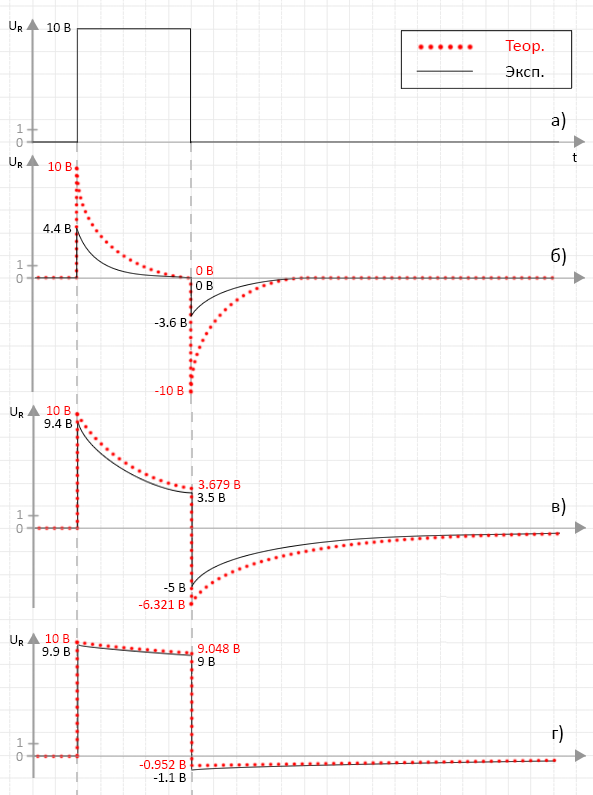
\includegraphics[width=14cm]{img/diff_with_theory2}
		\caption{Эксперементальная диаграмма входного и выходного импульса для дифференцирующей цепи при $R = 10$ кОм и: б) $C = 0.1$ нФ; в) $C = 1$ нФ; г) $C = 10$ нФ.} 
		\label{d:1} % название для ссылок внутри кода
	\end{center}
\end{figure}

\begin{figure}[H]
	\begin{center}
		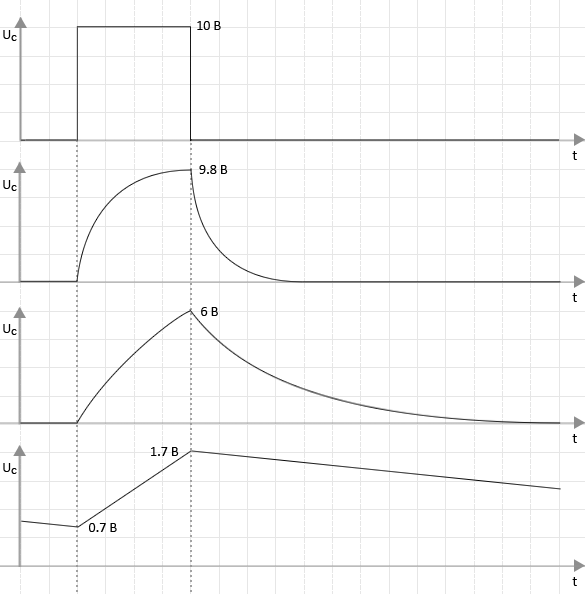
\includegraphics[width=14cm]{img/int}
		\caption{Эксперементальная диаграмма входного и выходного импульса для интегрирующей цепи при $R = 1$ кОм и: б) $C = 0.1$ нФ; в) $C = 1$ нФ; г) $C = 10$ нФ.} 
		\label{i:1} % название для ссылок внутри кода
	\end{center}
\end{figure}

\begin{figure}[H]
	\begin{center}
		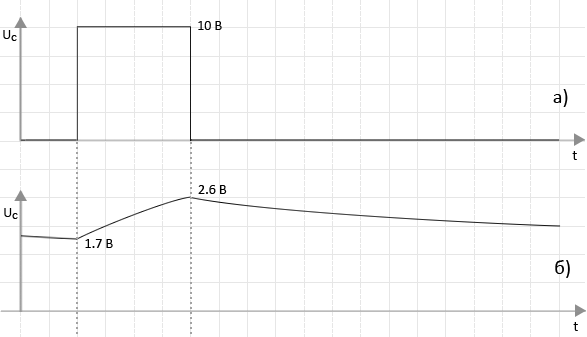
\includegraphics[width=14cm]{img/q5}
		\caption{Эксперементальная диаграмма входного и выходного импульса для интегрирующей цепи при $R = 1$ кОм, $C = 10$ нФ и $Q = 5$.} 
		\label{i:2} % название для ссылок внутри кода
	\end{center}
\end{figure}

\begin{figure}[H]
	\begin{center}
		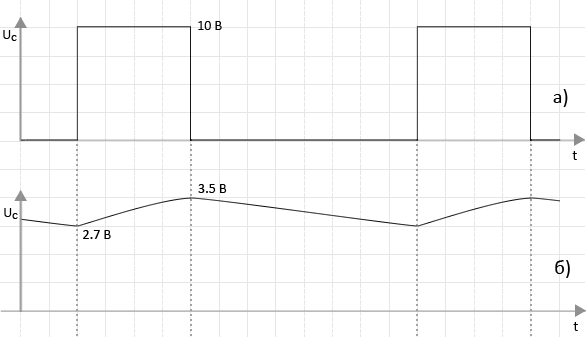
\includegraphics[width=14cm]{img/q3}
		\caption{Эксперементальная диаграмма входного и выходного импульса для интегрирующей цепи при $R = 1$ кОм, $C = 10$ нФ и $Q = 3$.}
		\label{i:3} % название для ссылок внутри кода
	\end{center}
\end{figure}

\section{Погрешности}

Рассчитаем отклонение эксперементально полученных данных от теоретических по формуле:

\begin{equation}
		\epsilon = |\frac{U\text{теор}-U\text{эксп}}{U\text{теор}}|
\end{equation}

\subsection{Дифференцирующая цепь}
\subsubsection{C = 0.1 нФ}
\begin{itemize}
\item[] а) $t = 0$: $\epsilon = |\frac{3.68 - 4.4}{ 3.68 }| * 100\% = 19 \%$

\item[] б) $t = t_\text{имп} - 0$: $\epsilon = |\frac{0 - 0}{ 0 }| * 100\% = 0 \%$

\item[] в) $t = t_\text{имп} + 0$: $\epsilon = |\frac{-3.28 - (-3.6)}{ -3.28 }| * 100\% = 10 \%$ 
\end{itemize}

\subsubsection{C = 1 нФ}
\begin{itemize}
\item[] а) $t = 0$: $\epsilon = |\frac{9.05 - 9.4}{ 9.05 }| * 100\% = 4 \%$

\item[] б) $t = t_\text{имп} - 0$: $\epsilon = |\frac{3.68 - 3.5}{ 3.68 }| * 100\% = 5 \%$

\item[] в) $t = t_\text{имп} + 0$: $\epsilon = |\frac{-5.37 - (-5)}{ -5.37 }| * 100\% = 7 \%$
\end{itemize}

\subsubsection{C = 10 нФ}
\begin{itemize}
\item[] а) $t = 0$: $\epsilon = \frac{| 9.05 - 9.4 |}{ 9.05 } * 100\% = 4 \%$

\item[] б) $t = t_\text{имп} - 0$: $\epsilon = \frac{| 3.68 - 3.5 |}{ 3.68 } * 100\% = 5 \%$

\item[] в) $t = t_\text{имп} + 0$: $\epsilon = \frac{| -0.86 - (-1.1) |}{ -0.86 } * 100\% = 27 \%$
\end{itemize}

\subsection{TODO Интегрируюшая цепь}
\subsubsection{C = 0.1 нФ}
\begin{itemize}
\item[] а) $t = 0$: $\epsilon = |\frac{3.68 - 4.4}{ 3.68 }| * 100\% = 19 \%$

\item[] б) $t = t_\text{имп} - 0$: $\epsilon = |\frac{0 - 0}{ 0 }| * 100\% = 0 \%$

\item[] в) $t = t_\text{имп} + 0$: $\epsilon = |\frac{-3.28 - (-3.6)}{ -3.28 }| * 100\% = 10 \%$ 
\end{itemize}

\subsubsection{C = 1 нФ}
\begin{itemize}
\item[] а) $t = 0$: $\epsilon = |\frac{9.05 - 9.4}{ 9.05 }| * 100\% = 4 \%$

\item[] б) $t = t_\text{имп} - 0$: $\epsilon = |\frac{3.68 - 3.5}{ 3.68 }| * 100\% = 5 \%$

\item[] в) $t = t_\text{имп} + 0$: $\epsilon = |\frac{-5.37 - (-5)}{ -5.37 }| * 100\% = 7 \%$
\end{itemize}

\subsubsection{C = 10 нФ}
\begin{itemize}
\item[] а) $t = 0$: $\epsilon = \frac{| 9.05 - 9.4 |}{ 9.05 } * 100\% = 4 \%$

\item[] б) $t = t_\text{имп} - 0$: $\epsilon = \frac{| 3.68 - 3.5 |}{ 3.68 } * 100\% = 5 \%$

\item[] в) $t = t_\text{имп} + 0$: $\epsilon = \frac{| -0.86 - (-1.1) |}{ -0.86 } * 100\% = 27 \%$
\end{itemize}

\subsubsection{C = 10 нФ, Q = 5}

\subsubsection{C = 10 нФ, Q = 3}
  
\section{Выводы}


\end{document}
